\chapter{Scanner}\label{chap:intro}

\lipsum[1]{}

\begin{lstlisting}[language=C++,numbers=none,caption=Die main() Methode,label=lst:ex1]
  #include "Scanner/Scanner/scanner.h"

  int main(int argc, char** argv) {
      if (argc != 2) {
          cout << "Missing argument." << endl;
      } else {
          char *filePath = argv[1];
          Scanner *sc = new Scanner(filePath);

          // Read all the tokens
          Token token;
          while (!token.isEOF()) {
              token = sc->nextToken();
              cout << token.getTypeString() << endl;
          }
      }
      return 0;
  }

}
\end{lstlisting}

\section{Bauen der Anwendung}
\lipsum{}

\begin{figure}[!htb]
    \centering
      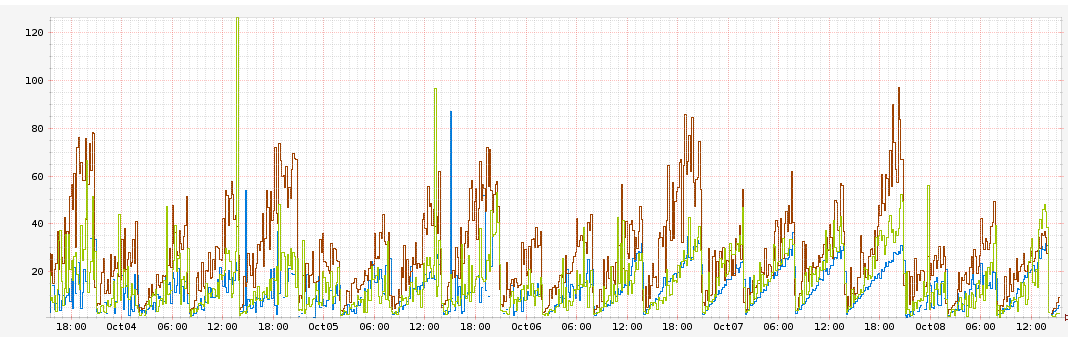
\includegraphics[width=0.85\linewidth]{example-graph.png}
    \caption{Eine Beispielstatistik}{Bildquelle:~\cite{JavaBeginner-Binding}}\label{fig:example}
\end{figure}

\lipsum{}
\section{References}

Literatur:~\cite{Example}

Look at~\ref{sec:objekthierarchie}

Example link to listing~\ref{lst:ex1}

And an example footnote\footnote{Look at this webpage: \url{https://www.google.com}}

\lipsum[2-3]{}% chktex 8
